\subsection*{Titration Series Validation}

To validate the two-sample titration dataset for use in abundance
assessment we evaluated two assumptions about the titrations. The first assumption was that the 
samples were mixed volumetrically in a \(log_2\) dilution series
according to the mixture design. To validate the sample volumetric mixing exogenous
DNA (ERCC plasmids) were spiked into the unmixed samples before mixing and quantified
using qPCR. The second assumption was that the unmixed PRE and POST samples
have the same proportion of prokaryotic DNA. The stool samples used to
generate the mixtures have both eukaryotic (primarily human) DNA and
prokaryotic DNA. If the proportion of prokaryotic DNA differs between
the unmixed samples, then the amount of DNA from the unmixed samples in
a titration targeted by 16S rRNA gene sequencing is not consistent with
the mixture design. To evaluate if the PRE and POST samples had the same
proportion of prokaryotic DNA total prokaryotic DNA in the titrations
samples were quantified using a qPCR assay targeting the 16S rRNA gene.


\subsubsection*{Spike-in qPCR results}

Titration series volumetric mixing was validated using qPCR to quantify exogenous
DNA (ERCC plasmids) spiked into the POST samples prior to mixing. 
The expectation is that the ERCC plasmid copy number will change at a rate consistent 
with the change in proportion of POST along  the titration series (Fig. \ref{fig:countExperimentalDesign}B). 
For our \(log_2\) two-sample-titration mixture design the expected slope of the
regression line between titration factor and Ct is 1, corresponding to a
doubling in template DNA every PCR cycle. The qPCR assay
standard curves had a high level of precision with \(R^2\) values close
to 1 and amplification efficiencies between 0.84 and 0.9 for all
standard curves indicating the assays were suitable for validating the
titration series volumetric mixing (Table \ref{tab:erccTable}).The qPCR assays targeting the
ERCCs spiked into the POST samples had \(R^2\) values and slope
estimates close to 1 (Table \ref{tab:erccTable}). Slope estimates less
than one were attributed to assay standard curve efficiency less than 1
(Table \ref{tab:erccTable}). ERCCs were also spiked into PRE samples but were not used
to validate volumetric mixing as PRE sample proportion differences were
too small for qPCR quantification. The expected difference for
the entire range of PRE concentrations is 1 \(C_t\). When considering the
quantitative limitations of the qPCR assay these results confirm that
the unmixed samples were volumetrically mixed according to the
two-sample titration mixture design.

\begin{table}

\caption{\label{tab:erccTable}ERCC Spike-in qPCR assay information and summary statistics. ERCC is the ERCC identifier for the ERCC spike-in, Assay is TaqMan assay, and Length and GC are the size and GC content of the qPCR amplicon.  The Std. $R^2$ and Efficiency (E) statistics were computed for the standard curves. $R^2$ and slope for titration qPCR results for the titration series.}
\centering
\begin{tabular}[t]{lllrrrrr}
\toprule
Subject & ERCC & Assay & Length & Std. $R^2$ & E & $R^2$ & Slope\\
\midrule
E01JH0004 & 012 & Ac03459877-a1 & 77 & 0.9996 & 86.19 & 0.98 & 0.92\\
E01JH0011 & 157 & Ac03459958-a1 & 71 & 0.9995 & 87.46 & 0.95 & 0.90\\
E01JH0016 & 108 & Ac03460028-a1 & 74 & 0.9991 & 87.33 & 0.95 & 0.84\\
E01JH0017 & 002 & Ac03459872-a1 & 69 & 0.9968 & 85.80 & 0.89 & 0.93\\
E01JH0038 & 035 & Ac03459892-a1 & 65 & 0.9984 & 86.69 & 0.95 & 0.94\\
\bottomrule
\end{tabular}
\end{table}


\subsubsection*{Prokaryotic DNA Concentration}

\begin{figure}
\centering
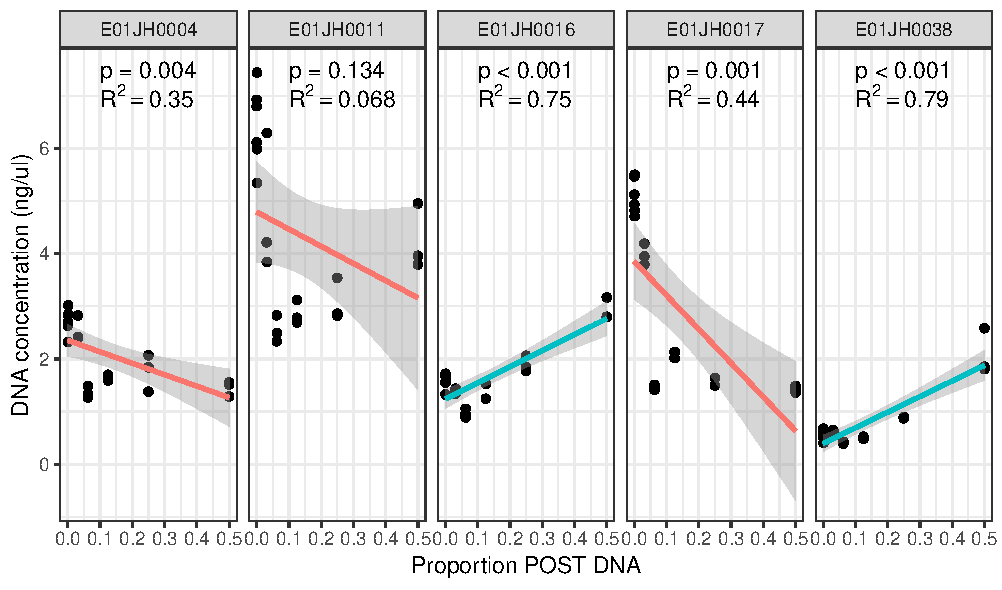
\includegraphics{bacPlot-1.pdf}
\caption{\label{fig:bacPlot}Prokaryotic DNA concentration (ng/ul) across
titrations measured using a 16S rRNA qPCR assay. \(R^2\) and p-values are shown linear models fit to prokaryotic DNA concentration versus proportion post DNA for each individual. 
Red lines indicate negative slope estimates and blue lines positive slope estimates.
p-value indicates significant difference from the expected slope of 0.
The grey regions indicate the linear model 95\% confidence interval.
Multiple test correction was performed using the Benjamini-Hochberg
method. One of the E01JH0004 PCR replicates for titration 3
(\(\theta=0.125\)) was identified as an outlier, with a prokaryotic DNA concentration of
0.003 ng/ul, and was excluded from the linear model. The linear model slope
was still significantly different from 0 when the outlier was included.}
\end{figure}

Observed changes in prokaryotic DNA concentration across titrations
indicate the proportion of prokaryotic DNA from the unmixed PRE and POST
samples in a titration is inconsistent with the mixture design (Fig.
\ref{fig:bacPlot}). A qPCR assay targeting the 16S rRNA gene was used to
quantify the concentration of prokaryotic DNA in the titrations. An
in-house standard curve with concentrations of 20 ng/ul, 2ng/ul, and 0.2
ng/ul was used, with efficiency 91.49, and \(R^2\) 0.999. If the
proportion of prokaryotic DNA is the same between PRE and POST samples
the slope of the concentration estimates across the two-sample titration
would be 0. For subjects where the proportion of prokaryotic DNA is
higher in the PRE samples, the slope will be negative, and positive when
the proportion is higher for POST samples. The slope estimates are
significantly different from 0 for all subjects excluding E01JH0011
(Fig. \ref{fig:bacPlot}). These results indicate that the proportion of
prokaryotic DNA is lower in POST when compared to the PRE samples for
E01JH0004 and E01JH0017 and higher for E01JH0016 and E01JH0038.




%% Discussion - Qualitative Assessment and Sparsity


\textbf{False positive features provide an explanation for Mothur and QIIME
pipelines having lower proportion of unmixed- and titration-specific
features not explained by sampling but high sparsity (Fig.
\ref{fig:qualPlot} and Table \ref{tab:pipeQA}). The statistical tests
used to determine if the specific features could be explained by
sampling alone only considers feature abundance. Therefore, the
statistical test is not able to distinguish between true low abundance
unmixed- and titration-specific features and low abundance sequence
artifacts. Mothur and QIIME count tables have ten times and three times
more features compared to DADA2, respectively (Table \ref{tab:pipeQA}).
While microbial abundance distributions are known to have long tails, it
is likely that the observed sparsity is an artifact of the 16S rRNA
sequencing measurement process. Similarly, significantly more features
than expected are commonly observed for mock community benchmarking
studies evaluating the QIIME and Mothur pipelines
\cite{kozich2013development}.

False positive features can be reduced, but not eliminated, using
smaller amplicon and prevalence filtering. The 16S rRNA region sequenced
in the study is larger than the region the \emph{de-novo}, and open
clustering pipelines were developed for, potentially explaining the
higher than expected sparsity \cite{kozich2013development}. Kozich et
al. \cite{kozich2013development} reduced the sequence error rate from
0.29\% to 0.06\% by using paired-end reads that completely overlap. The
larger region used in this study has a smaller overlap between the
forward and reverse reads. As a result, merging the forward and reverse
reads did not allow for sequence error correction that occurs when a
smaller amplicon is used. However, even when targeting smaller regions
of the 16S rRNA gene both the \emph{de-novo} (Mothur) and open-reference
clustering (QIIME) pipelines produced count tables with significantly
more features than expected in evaluation studies using mock
communities. Prevalence filtering is used to exclude low abundance
features, predominantly measurement artifacts \cite{callahan2016}. For
example, a study exploring the microbial ecology of the Red-necked stint
\emph{Calidris ruficollis}, a migratory shorebird, used a hard filter to
validate their study conclusions are not biases by false positive
features. The study authors compared results with and without prevalence
filter ensuring that the study conclusions were not biased by using the
arbitrary filter or including the low abundant features
\cite{risely2017gut}.}